\documentclass[bigger]{beamer}
\usepackage[utf8]{inputenc}
\usepackage[T1]{fontenc}
\usepackage{graphicx}
\usepackage{grffile}
\usepackage{longtable}
\usepackage{wrapfig}
\usepackage{rotating}
\usepackage[normalem]{ulem}
\usepackage{amsmath}
\usepackage{textcomp}
\usepackage{amssymb}
\usepackage{capt-of}
\usepackage{lmodern}
\usepackage{hyperref}
\usepackage{pdfpc-commands}
\usepackage{utils/kky}
\usepackage{multimedia}

\AtBeginSection[]
{
  \begin{frame}
    \tableofcontents[currentsection]
  \end{frame}
}


\defbeamertemplate*{title page}{customized}[1][]
{
  \usebeamerfont{title}\inserttitle\par
  \usebeamerfont{subtitle}\usebeamercolor[fg]{subtitle}\insertsubtitle\par
  \bigskip
  \usebeamerfont{author}\insertauthor\par
  \usebeamerfont{institute}\insertinstitute\par
  \usebeamerfont{date}\insertdate\par
  \usebeamercolor[fg]{titlegraphic}\inserttitlegraphic
}

\usetheme{Madrid}
\author[Hugo Richard]{Hugo Richard}
\date[\today]{}
\institute[Inria]{
  $\begin{array}{l}
     \includegraphics[height=1cm]{utils/inria.png} \end{array} \enspace
   \enspace \enspace \enspace $
   $\begin{array}{l} \includegraphics[height=1cm]{utils/ups.png} \end{array}$
}
\title[PhD Defense]{Unsupervised component analysis for neuroimaging data}
\titlegraphic{

\tiny{
  \vspace{-0.5cm}
\begin{tabular}{lll}
  \textbf{PHD supervisor}
  & Prof. Bertrand Thirion &\textit{ Inria, Université Paris-Saclay}\\
  && \\
  \textbf{Reviewers} & Prof. Tülay Adali &\textit{  University of Maryland Baltimore County }\\
  & Prof. Moritz Grosse-Wentrup &\textit{ University of Vienna }\\
  && \\
  \textbf{Examinators} & Prof.  Christian Jutten &\textit{ Université Grenoble Alpes }\\
  & Prof. Sylvain Chevalier &\textit{ Université de Versailles Saint-Quentin }\\
  &Prof. Matthieu Kowalski &\textit{ Université Paris Sud }\\
  & Prof. Aapo Hyvärinen &\textit{ University of Helsinki }\\
  &Prof. Alexandre Gramfort&\textit{ Inria, Université Paris-Saclay}\\

\end{tabular}
}}
  \setbeamertemplate{navigation symbols}{}

\begin{document}

\maketitle
\begin{frame}{}
  \begin{textblock*}{0cm}(0.9cm,-0.3cm)
  \hspace*{-1cm}
  \includegraphics[scale=1, height=\paperheight]{neurospin.jpg}
  \end{textblock*}
\end{frame}

\begin{frame}{}
  \begin{textblock*}{0cm}(0.9cm,-0.3cm)
    \hspace*{-1cm}
    \includegraphics[scale=1, width=\paperwidth]{irm.jpg}
  \end{textblock*}
\end{frame}

\begin{frame}{}
  \begin{textblock*}{0cm}(-1cm,-0.3cm)
    \hspace*{-1cm}
    \inlineMovie[autostart]{localizer-cut.mp4}{localizer-013.jpeg}{height=\paperheight}
  \end{textblock*}
\end{frame}

\begin{frame}{General linear model}
\only<1>{
  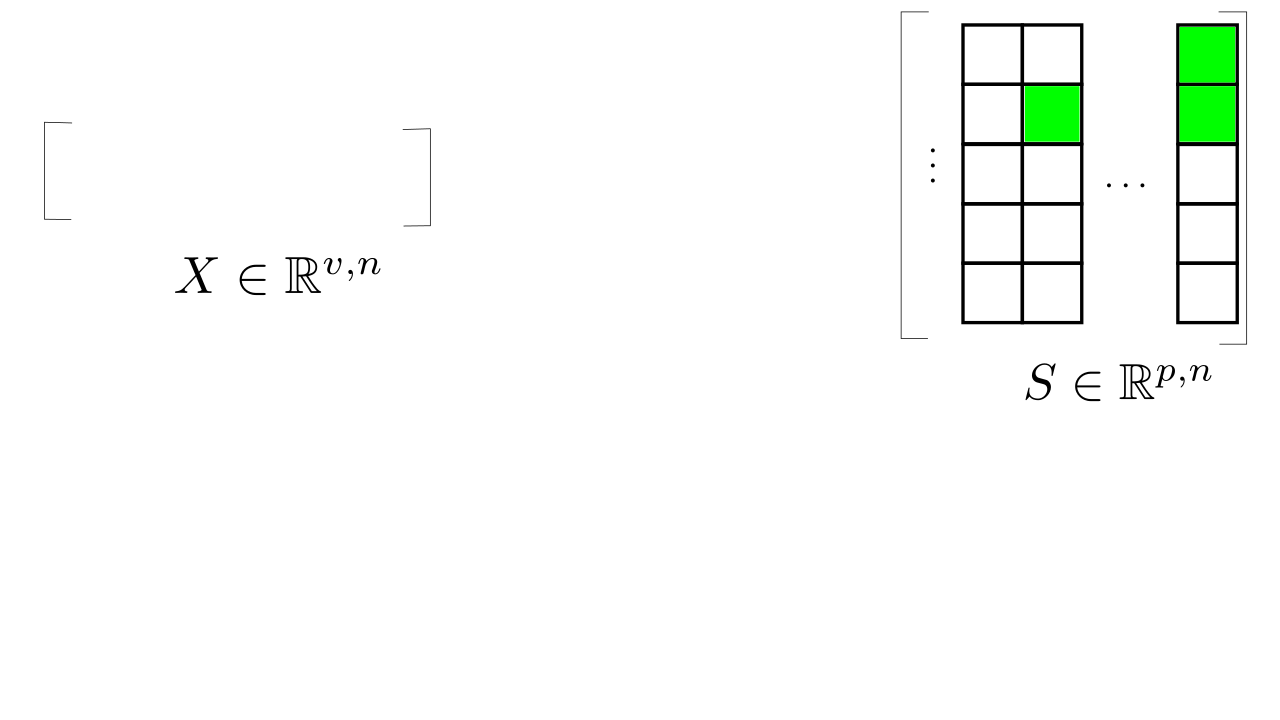
\includegraphics[scale=1, width=\textwidth]{glm1.png}
}
\only<2>{
  \includegraphics[scale=1, width=\textwidth]{glm2.png}
}

\only<3>{
  \includegraphics[scale=1, width=\textwidth]{glm3.png}
}

\only<4>{
  \includegraphics[scale=1, width=\textwidth]{glm4.png}
}

\only<5>{
  \includegraphics[scale=1, width=\textwidth]{glm5.png}
}

\only<6>{
  \includegraphics[scale=1, width=\textwidth]{glm6.png}
}
\end{frame}

\begin{frame}{General linear model}
  \begin{block}{One subject}
    \begin{equation*}
    X = A S + \mathrm{noise} 
    \end{equation*}
  \end{block}

  \pause

  \begin{block}{$m$ subjects}
    \begin{equation*}
      X_1 = A_1 S + \mathrm{noise} \enspace \enspace \cdots \enspace \enspace X_m = A_m S + \mathrm{noise}
    \end{equation*}
  \end{block}
  \pause
  
  \includegraphics[scale=0.20]{python/lr_button_0.png}
  \includegraphics[scale=0.20]{python/lr_button_1.png}
  \includegraphics[scale=0.20]{python/lr_button_2.png}
  \includegraphics[scale=0.20]{python/lr_button_3.png}
  \includegraphics[scale=0.20]{python/lr_button_4.png}
  \includegraphics[scale=0.20]{python/lr_button_5.png}
  \includegraphics[scale=0.20]{python/lr_button_6.png}
  \includegraphics[scale=0.20]{python/lr_button_7.png}
  \includegraphics[scale=0.20]{python/lr_button_8.png}
  \includegraphics[scale=0.20]{python/lr_button_9.png}
\end{frame}

\begin{frame}{}
  \begin{textblock*}{0cm}(-1cm,-0.3cm)
    \hspace*{-1cm}
  \inlineMovie[autostart]{raiders02-cut.mp4}{raiders02-001.jpeg}{height=\paperheight}
\end{textblock*}
\end{frame}


\begin{frame}
  \tableofcontents
\end{frame}

\section{Independent component analysis}
\begin{frame}{Sources and sensors}
  \centering
  \inlineMovie[loop&autostart]{source_emission.mp4}{source_emission-001.jpeg}{height=0.85\textheight}
\end{frame}
\begin{frame}{Mixing}
  \centering
  \inlineMovie[loop&autostart]{source_mixing.mp4}{source_mixing-001.jpeg}{height=0.85\textheight}
\end{frame}
\begin{frame}{Independent component analysis (noise-free)}
\begin{block}<1->{ICA model (Jutten, 1991)}
\begin{itemize}
\item Independent \emph{sources}: \(\sbb \in \mathbb{R}^{p}\)
\end{itemize}
\(p(\sbb) = p(s_1) \cdots p(s_p)\)
\begin{itemize}
\item \emph{\emph{Sensors}}: \(\xb \in \mathbb{R}^{p}\)
\end{itemize}

\centering
\emph{\emph{\(\xb = A\sbb\)}}

where \(A\) is the \emph{Mixing matrix}. 
\end{block}

\only<2>{
  $\begin{matrix} \includegraphics[width=6.2cm]{indet_1.pdf} \end{matrix}$ \hspace{0.5cm} $\begin{matrix} \includegraphics[width=5cm]{indet_2.pdf}\\  \includegraphics[width=5cm]{indet_3.pdf}\end{matrix}$
}
\begin{theorem}<3->[Identifiability of ICA (Common, 1994)]
  If \(\xb = A \sbb\) and \(\xb = A' \sbb'\)
  and if $\sbb$ has at most one Gaussian component,

Then 
\begin{itemize}
\item \(A = P A'\)
\item \(P\) is a scale and permutation matrix.
\end{itemize}
\end{theorem}
\end{frame}

\begin{frame}{Modeling complex stimuli}
  \begin{block}{ICA}
    \begin{equation*}
    X = AS
    \end{equation*}
    $\enspace $ S "as independent as possible"
  \end{block}

  \pause
  \begin{block}{Interpretation}
    \begin{itemize}
   \item $S \in \RR^{p, n}$: independent brain processes
   \item $A \in \RR^{v, p}$: corresponding spatial maps
     \end{itemize}
  \end{block}
  \pause
  \begin{block}{Dimension reduction}
    \begin{itemize}
    \item In ICA, we assume $p=v$.
    \item So we need to reduce the dimensionality of the data.
    \end{itemize}
  \end{block}

\end{frame}

\section{Group independent component analysis}
\begin{frame}{Group ICA}
\begin{block}{$m$ subjects exposed to the same stimuli}
  Consider $m$ subjects \(\xb_1, \dots, \xb_m \in \mathbb{R}^k\)
  such that \\ $\forall i \in \{1, \dots, m\}$:
  \begin{equation*}
  \xb_i = A_i \sbb + \nb_i
  \end{equation*}
\end{block}
\begin{block}{Interpretation}
  \begin{itemize}
  \item Shared sources $\sbb$: shared cognitive processes 
  \item Different mixing matrices $A_i$: different spatial topography of each subject
  \item Different noises $\nb_i$: deviation from the shared sources.
  \end{itemize}
\end{block}
\end{frame}

\begin{frame}{State of the art}
\begin{block}{ConcatICA [Calhoun, Adali, 2001]}
  \(\xb_1 \in \mathbb{R}^{k}, \xb_2 \in \mathbb{R}^{k}\)
  \begin{itemize}
  \item PCA of \(\xb = \begin{bmatrix} \xb_1 \\ \xb_2 \end{bmatrix}\)
  \end{itemize}
  \(\xb = \begin{bmatrix} U_1 \\ U_2 \end{bmatrix}  \xb_{red} \), 
  where \( \xb_{red}  \in \mathbb{R}^{k}\) and 
  \(\begin{bmatrix} U_1 \\ U_2 \end{bmatrix}\)
  is orthogonal.
  \begin{itemize}
  \item ICA of reduced data \( \xb_{red}  = A \sbb\)
  \end{itemize}
\end{block}
\pause
\begin{block}{CanICA [Varoquaux, 2010]}
  Replace PCA with (multi-set) CCA in ConcatICA \\
  CCA solves:
  $\begin{bmatrix} \EE[\xb_1 \xb_1^{\top}] & \EE[\xb_1 \xb_2^{\top}] \\
    \EE[\xb_2 \xb_1^{\top}] & \EE[\xb_2 \xb_2^{\top}]\end{bmatrix} \begin{bmatrix}
    \ub_1 \\ \ub_2 \end{bmatrix} =
  \lambda \begin{bmatrix} \EE[\xb_1 \xb_1^{\top}] & 0 \\
    0 & \EE[\xb_2 \xb_2^{\top}]\end{bmatrix} \begin{bmatrix}
    \ub_1 \\ \ub_2 \end{bmatrix}$
\end{block}
\end{frame}

\begin{frame}{State of the art}
  \begin{block}{About CanICA and ConcatICA}
    \begin{itemize}
    \item Very fast to fit
    \item Simple to implement
    \item Do not optimize a proper likelihood
    \end{itemize}
  \end{block}

\end{frame}


\begin{frame}{State of the art}
  \begin{block}{Typical noisy ICA likelihood [Moulines, Cardoso 1997]}
    \begin{itemize}
    \item $\xb_i = A_i \sbb + \nb_i, \nb_i \sim N(0, \sigma^2 I_{p})$
      $I_{p} \in \mathbb{R}^{p, p}$ is the identity matrix.
    \item \(p(\sbb) = d(s_1) \cdots d(s_p)\)
      
      Denoting $A = \begin{bmatrix} A_1 \\ \vdots \\ A_n \end{bmatrix}$, $\xb = \begin{bmatrix}
        \xb_1 \\ \vdots \\ \xb_n \end{bmatrix}$, we have
      \begin{align} p(\xb) &= \int p(\xb|\sbb)p(\sbb)d\sbb \\
                           &= \frac{1}{(2\pi \sigma^2)^{n/2}}\int e^{-\frac{1}{2 \sigma^2}||\xb - A \sbb||^2_2}p(\sbb)d\sbb
      \end{align}
    \item Intractable in general (it does not factorize)
    \end{itemize}
  \end{block}
\end{frame}

\begin{frame}{State of the art}
  \begin{block}{A Gaussian mixture model [Moulines, Cardoso 1997]}
    \begin{itemize}
    \item $\xb_i = A_i\sbb + \nb_i, \nb_i \sim N(0, \sigma^2 I_{k})$
     \item $p(s_j) = \frac1q \sum_{\alpha_j \in \mathcal{A}} p(s_j | \alpha_j)$
     \item $p(s_j | \alpha_j) = \mathcal{N}( s_j; 0, \alpha_j)$
    \end{itemize}
    where $\mathcal{A}$ is a known finite set.
  \end{block}
  \pause
  \begin{block}{Can we do an EM ?}
      $ \enspace \enspace \enspace \enspace p(\sbb | \xb, \alphab) =  \Ncal(\sbb, \mu_{\alphab}, \Sigma_{\alphab})$,
      where $\alphab = (\alpha_1, \dots, \alpha_p)$ \\
    and $V_{\alphab} = (\frac1{\sigma^2}A^{\top}A + \diag(\alphab)^{-1})^{-1}$, $\mu_{\alphab} = \frac1{\sigma^2}V_{\alphab} A^{\top} \xb$.
  \end{block}
  \pause
  \begin{block}{No we can't}
      $\enspace \enspace \enspace \enspace  p(\sbb | \xb) =  \sum_{\alphab \in \mathcal{A}^p} \Ncal(\sbb,
      \mu_{\alphab}, \Sigma_{\alphab})$ \\
    It is a sum with $q^p$ terms ($q=2, 3$, $p=20, 50$).
  \end{block}
  
\end{frame}

\begin{frame}{State of the art}
  \begin{block}{The model [Guo, 2008]}
    \begin{itemize}
    \item $\xb_i = A_i\sbb + \nb_i$
    \item $p(s_j) = \sum_{z=1}^q \Ncal(\mu_{zj}, \sigma_{zj})$
    \item $\mu_{zj}, \sigma_{zj}$ must be learned.
    \end{itemize}
  \end{block}

  It is even more difficult !
\end{frame}


\begin{frame}{State of the art}
  \begin{block}{Independent vector analysis [Lee, 2008]}
    \begin{itemize}
    \item $\xb_i = A_i \sbb_i$
    \item $\sbb_{[j]} = (s_{ij})_{i=1}^m$ are not independent
      \end{itemize}
  \end{block}

  \pause
  \begin{block}{Advantages}
    \begin{itemize}
  \item A closed form likelihood
  \item Takes naturally into account inter-subject variability
    \end{itemize}
  \end{block}

  \pause
  \begin{block}{Some instances of IVA}
    \begin{itemize}
  \item IVA-L [Lee, 2008]: $p_{\sbb_{[j]}}(\yb_{[j]}) \propto \exp(-\sqrt{\sum_i (y_{ij})^2})$
  \item IVA-G [Anderson, 2011] [Via, 2011]: $p_{\sbb_{[j]}}(\yb_{[j]}) = \Ncal( \yb_{[j]}; 0, \Sigma_j)$
  \item Many others: IVA-L-SOS [Bhinge, 2019]
    \end{itemize}
  \end{block}
  \pause
  No \emph{shared response}.
\end{frame}

\begin{frame}{State of the art}
  \begin{block}{Some other related work}
    \begin{itemize}
    \item Tensor ICA [Beckmann, 2005]
    \item SRM [Chen, 2015], FastSRM [Richard, Submitted to Aperture]
    \item Hyperalignment [Haxby, 2011]
    \end{itemize}
  \end{block}
\end{frame}


\section{MultiViewICA}
\label{sec:orgb958ef1}
\begin{frame}[label={sec:org65dfcba}]{Our contribution}
\begin{block}{Introducing MultiViewICA}
\begin{itemize}
\item A model with a closed form likelihood
\item A fast optimization algorithm
\item Theoretical guarantees
\item Improved source identification and localization
\end{itemize}
\end{block}
\end{frame}

\begin{frame}[label={sec:org10fe18b}]{Our contribution}
\begin{block}{Our model}
\(\xb_i \in \mathbb{R}^k, A_i \in \mathbb{R}^{k, k}\)
\begin{equation}
\boxed{
    \xb_i = A_i(\sbb + \nb_i), \enspace i=1,\dots, m
    }
\end{equation}

\begin{itemize}
\item Independent sources \(\sbb \in \mathbb{R}^k\)
\end{itemize}
\(p(\sbb) = d(s_1) \cdots d(s_k)\)
\begin{itemize}
\item Gaussian noise \(\nb_i \sim \mathcal{N}(0, \sigma^2 I_k)\)
\item Independent noise and independent from sources
\item Noise on the source side
\end{itemize}
\end{block}
\end{frame}

\label{sec:org55f3e63}
\begin{frame}[label={sec:org1ce1417}]{A closed-form likelihood}
\begin{example}[Typical noisy ICA likelihood (Bermond, Cardoso, 1999)]
\begin{itemize}
\item $\xb_i = A_i \sbb + \nb_i, \nb_i \sim N(0, \sigma^2 I_{k})$
  $I_{k} \in \mathbb{R}^{k, k}$ is the identity matrix.
\item \(p(\sbb) = d(s_1) \cdots d(s_k)\)
  
Denoting $A = \begin{bmatrix} A_1 \\ \vdots \\ A_n \end{bmatrix}$, $\xb = \begin{bmatrix}
  \xb_1 \\ \vdots \\ \xb_n \end{bmatrix}$, we have
\begin{align} p(\xb) &= \int p(\xb|\sbb)p(\sbb)d\sbb \\
                                &= \frac{1}{(2\pi \sigma^2)^{n/2}}\int e^{-\frac{1}{2 \sigma^2}||\xb - A \sbb||^2_2}p(\sbb)d\sbb
                                  \end{align}
\item Intractable in general (it does not factorize)
\end{itemize}
\end{example}
\end{frame}

\begin{frame}[label={sec:org89462cc}]{A closed-form likelihood}
\begin{block}{Our model}
\begin{itemize}
\item \(\xb_i = A_i(\sbb + \nb_i), \enspace i=1,\dots, m\)
\end{itemize}
\(\nb_{ik} \sim \mathcal{N}(0, \sigma^2)\), \(p(\sbb) = d(s_1) \cdots d(s_k)\) 
\end{block}
\begin{proof}[Closed form likelihood of our model]
\begin{itemize}
  \item Bla
\only<1>{\item $p(\xb) = \int p(\xb|\sbb)p(\sbb)d\sbb$}
\only<2-4>{\item $p(\xb) = \int $\textcolor{red}{$p(\xb|\sbb)$}\textcolor{blue}{$p(\sbb)$}$d\sbb$}
\only<5-9>{\item $p(\xb) = \int p(\xb|\sbb)p(\sbb)d\sbb$}
\only<3>{\item $p(\xb) = \int $\textcolor{red}{$ \prod_i p(\xb_i|\sbb)$}\textcolor{blue}{$\prod_j d(s_j)d\sbb$}}
\only<4>{\item $p(\xb) = \int $\textcolor{red}{$ \prod_i (|W_i| p^i_n(W_i\xb_i-\sbb))$}\textcolor{blue}{$\prod_j d(s_j)ds_j$}, $W_i = {A_i}^{-1}$}
\only<5-6>{\item $p(\xb) = \int \prod_i (|W_i|  $\textcolor{red}{$p^i_n(W_i\xb_i-\sbb)$}$)\prod_j d(s_j)ds_j$, $W_i = {A_i}^{-1}$}
\only<7-9>{\item $p(\xb) = \int \prod_i (|W_i| p^i_n(W_i\xb_i-\sbb))\prod_j d(s_j)ds_j$, $W_i = {A_i}^{-1}$}
\only<6>{\item $p(\xb) \propto \int \prod_i (|W_i| $\textcolor{red}{$
    \exp(-\frac{1}{2\sigma^2} \|W_i \xb_i - \sbb\|^2$} $)\prod_j
  d(s_j)ds_j$}
\only<7>{\item $p(\xb) \propto \int \prod_i (|W_i| $\textcolor{red}{$
    \exp(-\frac{1}{2\sigma^2} \|W_i \xb_i - \sbb\|^2$} $)\prod_j
  d(s_j)ds_j$}
\only<8>{\item $p(\xb) \propto \int \prod_i (|W_i| $\textcolor{red}{$
    \prod_j \exp(-\frac{1}{2\sigma^2} (\langle \wb_{ij} | \xb_i \rangle - s_j)^2$} $)\prod_j
  d(s_j)ds_j$}
\only<9>{\item $p(\xb) \propto \textcolor{red}{\int} \prod_i (|W_i|
  \textcolor{red}{\prod_j} \exp(-\frac{1}{2\sigma^2} (\langle \wb_{ij} | \xb_i \rangle - s_j)^2)
  \textcolor{red}{\prod_j} d(s_j)\textcolor{red}{ds_j}$}
\end{itemize}
\only<10>{
  $\mathcal{L} = -\sum_{i=1}^m \log|W_i| +
  \frac1{2\sigma^2}\sum_{i=1}^m\|W_i\xb_i - \tilde{\sbb}\|^2  +
  f(\tilde{\sbb})$
\begin{itemize}
\item $\tilde{\sbb} = \sum_{i=1}^n \frac{W_i\xb_i}{n}$
\item $f(s) = f(s_1) + \cdots f(s_k)$
\item $f$ is $d$ smoothed by a Gaussian kernel: $f(s_j) = \int\exp(-\frac{1}{2\sigma^2}m z^2)d(s_j - z)dz$
\end{itemize}
}
\end{proof}
\end{frame}

\label{sec:org6a44715}
\begin{frame}[label={sec:orgee78096}]{Optimization}
\begin{block}{Fast optimization}
\begin{itemize}
\item Alternate optimization (alternate between subjects)
\item Quasi newton with an approximation of the Hessian
\end{itemize}
\end{block}
\begin{block}{Quasi-Newton}
\begin{itemize}
\item Updates \(W_i = (I + \rho D)W_i\), \(D = {H_i}^{-1} G_i\) such that
\end{itemize}
\(\mathcal{L}((I + \varepsilon)W_i)) = \mathcal{L}(W_i) + <\varepsilon | G_i> +
<\varepsilon | H_i \varepsilon>, \enspace H_i \in \mathbb{R}^{k \times k \times k \times k}\)
\begin{align}
  \label{eq:hessian}
  \only<1>{(\mathcal{H}_i)_{abcd} &= \delta_{ad}\delta_{bc} + \delta_{ac}\left(\frac{1}{m^2}f''(\tilde{s}_a) + \frac{1 - 1/m}{\sigma^2}\right)y_{ib}y_{id} \\ & \text{where} \enspace \yb_i = W_i \xb_i}
                                                                                                                                                                \only<2>{(H_i)_{abcd} &= \delta_{ad}\delta_{bc} + \delta_{ac}\delta_{bd}\left(\frac{1}{m^2}f''(\tilde{s}_a) + \frac{1 - 1/m}{\sigma^2}\right)\left(y_{ib}\right)^2 \\ & \text{where} \enspace \yb_i = W_i \xb_i}
\end{align}
\begin{itemize}
\only<1>{\item $\mathcal{H}_i$ has $O(k^3)$ non zero coefficients.}
\only<2>{\item $H_i$ has $O(k^2)$ non zero coefficients. It is 2x2 block
  diagonal: easy to invert and regularize}

\end{itemize}
\end{block}
\end{frame}

\label{sec:org6e5f254}

\begin{frame}[label={sec:org50c428c}]{Theoretical contributions}
\begin{theorem}<+->[Identifiability of MultiViewICA]
\begin{itemize}
\item Consider \(\xb_i = A_i(\sbb + \nb_i), \enspace
  i=1,\dots, m\) \(\nb_i \sim \mathcal{N}(0, \sigma^2 I_k)\), \(p(\sbb) = d(s_1)
  \cdots d(s_k)\), $\sbb$ has at most one Gaussian component

\item Assume \(\xb_i = A'_i(\sbb' + \nb'_i), \enspace i=1,\dots, m\), \(\nb'_i
  \sim \mathcal{N}(0, \sigma'^2 I_k)\), \(p(\sbb') = d'(s'_1) \cdots d'(s'_k)\)
\end{itemize}

Then, \(\exists P\in \mathbb{R}^{k\times k}\) a scale and permutation matrix s.
t. \(\forall i \enspace A'_i = A_i P\).
\end{theorem}
\begin{theorem}<+->[Robustness to choice of hyperparameter \(\sigma\)]
\begin{itemize}
\item Assume sub-linear growth on \(f'\): \(|f'(x)|\leq c|x|^{\alpha} + d\) for
  some \(c, d > 0\) and \(0<\alpha<1\) (Verified in practice)
\item Assume that \(\xb_i\) follows the model with \(\sigma'\) and \(d'\).
\end{itemize}
Then, \(\exists \Lambda\) a diagonal matrix s.t. \((\Lambda (A^1)^{-1}, \dots, \Lambda (A^m)^{-1})\) is a stationary point of \(\mathcal{L}\).
\end{theorem}
\end{frame}

\begin{frame}{Small recap}
  \begin{block}{What do we have so far}
    \begin{itemize}
    \item A principled approach to perform GroupICA
    \item Theoretical guarantees
    \end{itemize}
  \end{block}
  \begin{block}{Some questions}
    \begin{itemize}
    \item Can we have a more general model while still keeping the likelihood in
      closed form ?
    \item How to deal with Gaussian sources ?
    \end{itemize}
  \end{block}
\end{frame}

\section{SharedICA}
\begin{frame}{Our contribution: Shared ICA (ShICA)}
  \begin{block}{ShICA model}
     \begin{center}$ \xb_i = A_i (\sbb + \nb_i)$ \end{center}
    \begin{itemize}
      \item $\nb_i \sim \Ncal(0, \Sigma_i)$ where $\Sigma_i$ is diagonal positive.
      \item $\sbb$ are independent components some of which may be Gaussian
     \end{itemize}
  \end{block}
  \begin{block}{ShICA-J: }
    \begin{itemize}
\item In theory Multiset CCA solves ShICA (under some conditions).
\item In practice, sampling noise causes some issues.
\item Joint diagonalization solves it: ShICA-J = MCCA + Joint diag
  \end{itemize}
  \end{block}
  \begin{block}{ShICA-ML}

    \begin{itemize}
  \item A maximum likelihood approach to ShICA
  \item ShICA-ML can separate Gaussian and non-Gaussian data
    \end{itemize}
  \end{block}
\end{frame}

\begin{frame}{ShICA is identifiable}
\begin{theorem}[Identifiability]
  We assume noise diversity in Gaussian components:
  Let $\mathcal{G}$ be the set of Gaussian components. For all $j, j'  \in \mathcal{G}, j \neq j'$, the sequences $(\Sigma_{ij})_{i=1 \dots m}$ and $(\Sigma_{ij'})_{i=1 \dots m}$ are different where $\Sigma_{ij}$ is the $j, j$ entry of $\Sigma_i$.

  Let $\Theta=(A_1, \dots, A_m, \Sigma_1, \dots,\Sigma_m)$ be the set of
  parameter that generates $\xb_1 ,\dots, \xb_m$ from the ShICA model. 
  We let $\Theta'=(A_1', \dots, A_m', \Sigma_1', \dots,\Sigma_m')$ another set
  of parameters, and assume that they also generate the data. Then, there exists a sign and permutation matrix $P$ such that for all $i$, $A_i'=A_iP$, and $\Sigma_i'= P^{\top} \Sigma_i P$.
\end{theorem}
Note that noise diversity in Gaussian component is also a necessary condition.
\end{frame}

\begin{frame}{Multiset CCA solves GroupICA}
  \begin{theorem}[Solving GroupICA with Multiset CCA]
    We assume $\xb_i$ follows $\xb_i = A_i (\sbb + \nb_i)$ where  $\nb_i \sim \Ncal(0, \Sigma_i)$ where $\Sigma_i$ is diagonal and consider the multiset CCA
    problem \\
      $C \ub = \lambda D \ub$ \\
      where block $i, j$ of $C$ is $\EE[\xb_i \xb_j^{\top}]$ and $D$ is block
      diagonal with block $i, i$ given by $\EE[\xb_i \xb_i^{\top}]$.
      Let $U = [\ub_1 \dots \ub_k] = \begin{bmatrix} W_1^{\top} \\ \vdots \\
        W_m^{\top} \end{bmatrix}$ where $W_i \in \RR^{k, k}$.  \\
      Then \underline{if $\lambda_1 \dots \lambda_k$ are distincts}, $W_i = P \Gamma_i A_i^{-1}$ where $P$ is a permutation matrix and
      $\Gamma_i$ a scaling matrix.  
  \end{theorem}
  Note that the distinct eigenvalue condition is also necessary.

  Note that the condition is stronger than noise diversity (we can exhibit an identifiable
  example on which MCCA fails).
\end{frame}

\begin{frame}{Practical issues with Multiset CCA}
    The mapping from matrices to eigenvectors is
    highly non smooth...
  \begin{block}{Practical example}
    $m=3$, $k=2$ and $\Sigma_i$ such that $\lambda_1 = 2 + \epsilon$ and $\lambda_2
    = 2$. \\
    $W_i$: Solution of multiset CCA on true covariance matrices $C_{ij}$ \\
    $\tilde{W}_i$: Solution of multiset CCA on perturbed covariance matrices 
    $\tilde{C}_{ij} = C_{ij} + \delta S$ where $S$ positive
    symmetric matrix of norm $1$.
  \end{block}
  \includegraphics[scale=0.8]{figures/multicca_gap.pdf}
\end{frame}

\begin{frame}{Solving practical issues with joint diagonalization}
  \begin{block}{Large gap between the first $k$ eigenvalues and others}
    $\lambda_k - \lambda_{k+1} > \frac{m-1}{1 + \max_{ij} \Sigma_{ij}} +
    \frac1{1 + \min_{ij} \Sigma_{ij}}$
  \end{block}
  \begin{block}{Practical implications}
    The span of the $p$ leading eigenvectors is preserved:
    $W_i \approx Q \tilde{W}_i$.
    We recover $Q$ by joint diagonalization of $Q \tilde{W}_i \frac1{n}X_i X_i^{\top} \tilde{W}_i^{\top}Q^{\top}$
  \end{block}
  \includegraphics[scale=0.8]{figures/multicca_gap_jd.pdf}
\end{frame}

\begin{frame}{ShICA-J}
 Use Multiset CCA and joint diagonalization to obtain $W_i$ up to a
    scaling $\Psi_i$.
  \begin{block}{Find the scalings}
    We solve $\min_{\Psi} \sum_{i \neq j} \|\Psi_i \diag(Q \tilde{W}_i
    \tilde{C}_{ij} \tilde{W}_j Q^{\top}) \Psi_j - I_k \|^2$.
    The estimates of $W_i$ are then given by $\hat{W}_i = \Psi_i Q \tilde{W}_i$.
  \end{block}

  \begin{block}{Find the noise variances}
    We use the maximum likelihood estimate of $\xb_i = \hat{W}_i^{-1}(\sbb +
    \nb_i)$ via an EM algorithm.
    The E-step and M-step are in closed form yielding a fast algorithm.
  \end{block}
  ShICA-J is very fast. But it is not a maximum likelihood estimator.
\end{frame}


\begin{frame}{ShICA-ML: the maximum likelihood estimator}
  \begin{block}{ShICA-ML}
      \centerline{$\xb_i = A_i (\sbb + \nb_i)$} where $\nb_i \sim \Ncal(0, \Sigma_i)$, $\Sigma_i$ diagonal and $s_j
  \sim \frac12 \sum_{\alpha \in \{ \frac12, \frac32 \}} \Ncal(0, \alpha)$.
  \end{block}

  \begin{block}{Optimization}
    Optimized via an EM algorithm.
    \vspace{-1em}
    \begin{align*}
      \text{E-step: } && \EE[\sbb | \xb] = \frac{\sum_{\alpha \in \{\frac12, \frac32
      \}}\theta_{\alpha} \eb_{\alpha}}{\sum_{\alpha \in
      \{\frac12, \frac32 \}}\theta_{\alpha}}
      && 
         \VV[\sbb | \xb] = \frac{\sum_{\alpha \in \{\frac12, \frac32
         \}}\theta_{\alpha} V_{\alpha}}{\sum_{\alpha \in
         \{\frac12, \frac32 \}}\theta_{\alpha}} 
    \end{align*}
    \vspace{-1em}

    $\eb_{\alpha}= \left(\sum_{i=1}^m \Sigma_i^{-1}  + \frac1{\alpha}I
    \right)^{-1}  \sum_{i=1}^m \left(\Sigma_i^{-1} W_i \xb_i \right)$,
    $V_{\alpha} = (\sum_{i=1}^m \Sigma_i^{-1}  + \frac1{\alpha}I)^{-1}$ and
    $\theta_{\alpha} = \mathcal{N}((\sum_{i=1}^m \Sigma_i^{-1})^{-1}
    \Sigma_i^{-1} \yb_i; 0, (\alpha I + (\sum_{i=1}^m
    \Sigma_i^{-1})^{-1})^{\frac12})$ \\
    M-step: Closed form updates for noise variances and quasi-newton updates for
    unmixing matrices.
  \end{block}
  ShICA-J provides a great initialization to ShICA-ML
\end{frame}

\begin{frame}{Synthetic experiments}
  \begin{block}{Separation performance depending on the density of sources}
  $m=4$ views, $k=5$ components, non-Gaussian sources are from a Laplace
  density, we use the ShICA model using: \\
  (a) Gaussian components with noise diversity \\
  (b) non-Gaussian components without noise diveristy \\
  (c) Half of components are Gaussian with noise diversity, the other half is
  non-Gaussian without diversity
\end{block}
  \begin{center}
    \includegraphics[width=\textwidth]{./figures/identifiability.pdf}
  \end{center}
\end{frame}

\begin{frame}{Synthetic experiments}
  \begin{block}{Computation time}
    We generate components from a slightly super-Gaussian density $s_j = d(x)$
    with $d(x) = x |x|^{0.2}$ and $x \sim \mathcal{N}(0, 1)$ vary the number of
    samples $n=10^2 \dots 10^4$.
  \end{block}
  \begin{center}
    \includegraphics[width=0.65\textwidth]{./figures/synthetic_gaussian_timings.pdf}
  \end{center}
\end{frame}

\begin{frame}{Reconstruction experiment fMRI}

  \begin{columns}[T] % align columns
    \begin{column}{.4\textwidth}
      \begin{itemize}
      \item Train data: 100\% subjects 80\% runs -> Learn unmixing matrices
      \item Test data: 80\% subjects 20\% runs -> Compute sources
      \item Validation data: 20\% subjects 20\% runs -> Measure R2 score
      \end{itemize}
    \end{column}%
    \hfill%
    \begin{column}{.6\textwidth}
      \begin{center}
        \includegraphics[width=\linewidth]{./figures/reconstruction.pdf}
      \end{center}
    \end{column}%
  \end{columns}
\end{frame}

\begin{frame}{Timesegment matching fMRI}
  \begin{columns}[T] % align columns
    \begin{column}{.4\textwidth}
      \begin{itemize}
      \item Timesegment matching accuracy: Locate a 9 timeframes timesegment in a left out subject by correlation with the average response of other subjects.
      \item Train data: 80\% runs $\rightarrow$ Learn unmixing matrices
      \item Test data: 20\% runs $\rightarrow$ Measure accuracy
      \end{itemize}
    \end{column}%
    \hfill%
    \begin{column}{.6\textwidth}

      \begin{center}
        \includegraphics[width=\linewidth]{./figures/timesegment_matching.pdf}
      \end{center}
    \end{column}%
  \end{columns}
\end{frame}


\begin{frame}
  \begin{block}{MEG Phantom experiment}
    \begin{itemize}
    \item 8 dipoles in a plastic head at different locations
    \item Dipoles separately emit the same known signal $S_{true}$ during $n$ epochs
    \item $20$ sources estimated: the best one is compared with $S_{true}$
    \end{itemize}
  \end{block}
  \begin{center}
    \includegraphics[width=0.7\textwidth]{./figures/meg_phantom_neurips.pdf}
  \end{center}
\end{frame}

\section{Conclusion}
\begin{frame}{Conclusion}
\begin{block}{Take home message}
\begin{itemize}
\item ShICA is a powerful framework to extract shared sources
\item ShICA-J yields a fast approach but only uses second order information,
  ShICA-ML is a bit slower but uses in addition non-Gaussianity.
\item Yields better results in practice: extensive comparison on multiple
  neuroscience modalities.
\end{itemize}
\end{block}

\begin{block}{Future Work}
\begin{itemize}
  \item These methods work on reduced data. How to provide the best dimension
    reduction method ?
  \item The non-Gaussian density of the shared sources in ShICA-ML could be learned.  
\end{itemize}
\end{block}
\end{frame}

\begin{frame}{About us}
  \begin{block}{ICA may be old stuff but ideas can be reused}
    \begin{itemize}
    \item Our Hessian approximation is specific to ICA but a similar technique
      is used for Fast joint diagonalization.
     \item Multiplicative algorithms provide a way to ``remove the Jacobian term''
       when training deep generative neural networks''.
     \item ICA is done under orthogonal or invertible constrains on mixing
       matrices leading to optimization on Riemannian manifold. The natural
       gradient in ICA coincides with the relative gradient. In neural networks,
       such ideas are used to obtain \emph{equivariant} networks. 
     \end{itemize}
  \end{block}
\end{frame}

  \begin{frame}{About us}
  \begin{block}{Other contributions}
    \begin{itemize}
  \item Mvlearn: MultiView Machine Learning in Python (JMLR,
    2021 - non-first author)
  \item Brainiak: The brain imaging analysis kit (OSF,
    2020 - non-first author)
  \item Local optimal transport for functional brain template estimation (IPMI,
    2019 - non-first author)
  \item Optimizing deep video representation to match brain activity (CCN, 2018)
  \item A fast algorithm for performing dimension reduction under orthogonal
    constrains (srm) (OHBM, 2018)
    \end{itemize}
  \end{block}
\end{frame}

\end{document}
